\documentclass[11pt]{article}
\usepackage[utf8]{inputenc}
\usepackage[T1]{fontenc}
\usepackage[margin=1in]{geometry}
\usepackage{amsmath,amssymb}
\usepackage{graphicx}
\usepackage{booktabs}
\usepackage{authblk}
\usepackage[hidelinks]{hyperref}
\graphicspath{{./}{../figures/}}

\title{\bfseries Beyond the marginal distribution: long-range correlations in
prime gaps imprint on the 3D conformation of a self-avoiding polymer}
\author[1]{Ruqing Chen\thanks{Corresponding author: \texttt{ruqing@hotmail.com}}}
\affil[1]{GUT Geoservice Inc., Montreal, Quebec, Canada}
\date{\today}

\begin{document}
\maketitle

\begin{abstract}
The folding of a heteropolymer is governed by its monomer sequence, yet the
intermediate regime between periodic and random sequences---those that are
aperiodic but deterministic---remains largely unexplored. We introduce the
Prime-Driven Topological Polymer (PDTP), a coarse-grained self-avoiding chain in
which the local bending stiffness is set by an exponential map of the local prime
gap, so that dense prime clusters act as flexible hinges and the long inter-prime
runs as rigid rods. Using overdamped Langevin dynamics with simulated annealing,
we ask whether the folded state is fixed by the composition of this sequence or by
its arithmetic ordering. To separate the two, we compare the true prime chain
against surrogates that preserve the marginal stiffness distribution exactly while
destroying sequential order. The gross conformation is surrogate-invariant:
neither the radius of gyration nor the tail-weighted core--shell amplitude
distinguishes the true chain from a shuffle. The finer organization does: the
Spearman correlation between stiffness and radial position is significantly
suppressed for the true sequence ($\rho = +0.105$ vs.\ $+0.137$ at
$N = 4\times10^{4}$; $p = 6.5\times10^{-5}$, $d = -0.96$), an effect a
decomposition attributes to ordering rather than to the gap distribution. The
imprint is quantitatively modest ($\sim\!1\%$ of the radial-rank variance) but
statistically robust and reproducible across system sizes, demonstrating that
deterministic arithmetic order leaves a measurable trace on three-dimensional
structure---one that survives the entropically favored radial sorting of the
collapse.
\end{abstract}

\section{Introduction}

The folding of a heteropolymer into a compact, organized state is a canonical
problem of soft-matter physics, underlying phenomena from protein structure to
chromatin architecture~\cite{deGennes,LiebermanAiden}. A primary determinant of
the emergent morphology is the monomer sequence---the one-dimensional arrangement
of chemically or mechanically distinct units along the
backbone~\cite{Pande}. Two limiting classes of sequence have been studied in
depth. At one extreme lie deterministic \emph{periodic} sequences, epitomized by
block copolymers, whose translational symmetry drives microphase separation into
lamellar, cylindrical, and related ordered mesophases~\cite{Leibler,Bates}. At the
other extreme lie \emph{random} heteropolymers, in which the sequence is a quenched
realization of uncorrelated disorder and the folding landscape is governed by
frustration and glassy statistics~\cite{Bryngelson,Garel}. Between these poles lies
a comparatively unexplored regime: sequences that are neither periodic nor random,
but \emph{aperiodic and deterministic}, carrying long-range correlations of purely
structural origin. How such long-range-ordered aperiodicity is expressed in the
three-dimensional conformation of a collapsed chain remains largely open.

Number theory has repeatedly furnished physics with precisely this kind of
structured aperiodicity. The statistics of the nontrivial zeros of the Riemann
zeta function coincide with the spectral fluctuations of random-matrix ensembles,
forming a celebrated bridge between arithmetic and quantum
spectra~\cite{Montgomery,BerryKeating}. In real space, aperiodic tilings and
quasicrystals demonstrate that deterministic, non-periodic order can generate sharp
diffraction and hierarchical organization absent from both crystals and
glasses~\cite{Shechtman,Levine}. The sequence of prime numbers occupies a
distinctive place in this landscape: it is fully deterministic yet globally
aperiodic, its coarse density decays only logarithmically as dictated by the prime
number theorem, and its local structure---encoded in the sequence of prime gaps
$g_i$, the distances between consecutive primes---carries well-documented
correlations that are neither periodic nor memoryless~\cite{HardyWright,Cramer}.
These properties make the prime-gap sequence a natural candidate for a designed,
deterministic constraint to be mapped onto physical space, in the same spirit that
quasiperiodic order has been imprinted onto photonic and mechanical
metamaterials~\cite{Macia}.

We realize this mapping mechanically. In the Prime-Driven Topological Polymer
(PDTP), each bead $i$ of a coarse-grained bead--spring chain is assigned a local
bending stiffness that is an exponential function of its prime gap [Eq.~(1)]. Dense
clusters of primes (short gaps) become flexible hinges, while the rare long gaps
become nearly rigid rods. Upon collapse, this construction establishes a
competition between two tendencies. The first is generic to any stiff--flexible
copolymer: excluded-volume repulsion and bending energy tend to expel rigid
segments toward the periphery while flexible segments accommodate the curvature of
the dense core, yielding a positive correlation between local stiffness and radial
position~\cite{KratkyPorod,Montesi}. The second is specific to the arithmetic
origin of the sequence: the deterministic ordering of the gaps along the
backbone constrains which segments can reach the surface. The central question is
whether this arithmetic ordering leaves any measurable imprint on the folded state,
or whether the conformation is fixed entirely by the \emph{marginal} distribution
of stiffnesses, indifferent to their sequence. To resolve this we introduce a
surrogate-based null model that preserves the marginal distribution exactly while
destroying sequential order, and show---through a large ensemble of annealed
trajectories---that the arithmetic ordering does leave a small but statistically
robust signature, invisible in gross morphology and in marginal-matched nulls, yet
detectable in the rank organization of the collapse.

\section{Model definition}

\subsection{Prime skeleton and gap extraction}
We identify the beads of a chain of length $N$ with the integers
$i = 0,1,\dots,N-1$. A sieve of Eratosthenes partitions these indices into primes
and composites~\cite{HardyWright}. For a composite bead lying in the maximal run of
consecutive composites bounded by the primes $p_{\text{left}} < i < p_{\text{right}}$
we define a \emph{local prime gap} $g_i = p_{\text{right}} - p_{\text{left}}$,
assigning every bead within a given inter-prime run the same value; for a prime bead
$g_i = 0$. The boundary segments take $g_i = p_1$ for $i < p_1$ and
$g_i = N - p_{\text{last}}$ for $i > p_{\text{last}}$. Within our largest system,
$N = 4\times10^4$, the extremal gap is $g_{\max} = 72$, between the primes $31397$
and $31469$.

\subsection{Gap-driven exponential stiffness}
The gap field is mapped onto the local bending stiffness $k_i$ through a saturated
exponential map,
\begin{equation}
k_i =
\begin{cases}
k_{\text{hinge}}, & i \ \text{prime},\\[3pt]
\min\!\left[\, k_{\text{hinge}}\, e^{\alpha g_i},\; k_{\max}\,\right], & i \ \text{composite}.
\end{cases}
\end{equation}
The exponential rather than linear map is essential: because the gap envelope varies
only slowly, a linear coupling produces a stiffness field too smooth to break the
conformational symmetry, whereas the exponential map converts modest gap fluctuations
into a stiffness contrast spanning nearly four orders of magnitude
($k_{\max}/k_{\text{hinge}} = 2000$ at our parameters). The amplification coefficient
$\alpha$ and cap $k_{\max}$ are fixed by an independent stability calibration
(Sec.~\ref{sec:calib}).

\subsection{Coarse-grained potential energy}
Bonds between consecutive beads are harmonic,
\begin{equation}
E_{\text{bond}} = \tfrac{1}{2} k_{\text{bond}} \sum_{i=1}^{N-1}
\big(\lvert \mathbf{r}_i - \mathbf{r}_{i-1}\rvert - b_0\big)^2 ,
\end{equation}
with rest length $b_0$. The gap-driven stiffness enters through a cosine bending
potential on interior triplets,
\begin{equation}
E_{\text{bend}} = \sum_{i=1}^{N-2} k_i \left(1 - \cos\theta_i\right),\qquad
\cos\theta_i = \frac{(\mathbf{r}_i-\mathbf{r}_{i-1})\cdot(\mathbf{r}_{i+1}-\mathbf{r}_i)}
{\lvert\mathbf{r}_i-\mathbf{r}_{i-1}\rvert\,\lvert\mathbf{r}_{i+1}-\mathbf{r}_i\rvert},
\end{equation}
so that $k_i$ acts as a local, sequence-dependent bending modulus~\cite{KratkyPorod,Montesi}.
Self-avoidance is a purely repulsive Weeks--Chandler--Andersen (WCA) interaction
between non-bonded pairs ($\lvert i-j\rvert > 1$)~\cite{WCA},
\begin{equation}
E_{\text{WCA}}(r) =
\begin{cases}
4\varepsilon\!\left[(\sigma/r)^{12}-(\sigma/r)^{6}\right] + \varepsilon, & r < r_c = 2^{1/6}\sigma,\\[3pt]
0, & r \ge r_c,
\end{cases}
\end{equation}
evaluated with a $k$-d-tree neighbor list and with the pairwise force magnitude
capped at $f_{\text{cap}}^{\text{WCA}}$ as a numerical safeguard. Finally, a weak
radial restoring force tethers each bead to the instantaneous center of mass
$\mathbf{r}_{\mathrm{cm}}$,
\begin{equation}
\mathbf{F}^{\text{conf}}_i = -\,k_{\text{conf}}\,(\mathbf{r}_i - \mathbf{r}_{\mathrm{cm}}),
\end{equation}
with $k_{\text{conf}}$ small: it gathers the globule without crushing the rigid rods,
allowing the gap-driven gradient to survive collapse.

\subsection{Overdamped Langevin dynamics and annealing}
The chain is propagated with overdamped (Brownian) Langevin dynamics in reduced
units ($\sigma = \varepsilon = k_B = 1$)~\cite{Ermak}:
\begin{equation}
\mathbf{r}_i \leftarrow \mathbf{r}_i + \mu\,\mathbf{F}_i\,\Delta t
+ \sqrt{2\mu\, k_B T\, \Delta t}\;\boldsymbol{\xi}_i,\qquad
\boldsymbol{\xi}_i \sim \mathcal{N}(\mathbf{0}, \mathbb{I}_3),
\end{equation}
where $\mathbf{F}_i = -\nabla_i E$, $\mu$ is the mobility, and $\boldsymbol{\xi}_i$
is independent Gaussian noise. Compaction is achieved by simulated
annealing~\cite{Kirkpatrick}, lowering the temperature geometrically,
\begin{equation}
k_B T(t) = k_B T_{\text{hi}} \left(T_{\text{lo}}/T_{\text{hi}}\right)^{t/(n_{\text{steps}}-1)} .
\end{equation}
Per-bead displacements are capped at $\lvert\Delta\mathbf{r}_i\rvert \le \delta_{\max}$,
and each trajectory is initialized as a correlated random walk (persistence $0.55$).
Parameters are listed in Table~\ref{tab:params}.

\begin{table}[htbp]
\centering
\caption{Model and protocol parameters (reduced units).}
\label{tab:params}
\begin{tabular}{lll}
\toprule
Symbol & Value & Meaning \\
\midrule
$b_0$ & $1.0$ & bond rest length \\
$k_{\text{bond}}$ & $45.0$ & bond stiffness \\
$k_{\text{hinge}}$ & $0.25$ & baseline (prime) bending stiffness \\
$\alpha$ & $0.15$ & gap amplification coefficient (calibrated) \\
$k_{\max}$ & $500.0$ & bending-stiffness cap (calibrated) \\
$\sigma,\ \varepsilon$ & $1.0,\ 1.0$ & WCA diameter, energy scale \\
$r_c$ & $2^{1/6}\sigma$ & WCA cutoff \\
$f_{\text{cap}}^{\text{WCA}}$ & $30.0$ & WCA force cap \\
$k_{\text{conf}}$ & $0.02$ & weak confinement constant \\
$\mu$ & $1.0$ & mobility \\
$\Delta t$ & $0.008$ & integration step \\
$\delta_{\max}$ & $0.25$ & per-bead displacement cap \\
$k_B T_{\text{hi}},\ k_B T_{\text{lo}}$ & $0.50,\ 0.003$ & annealing temperature range \\
\bottomrule
\end{tabular}
\end{table}

\begin{figure}[htbp]
\centering
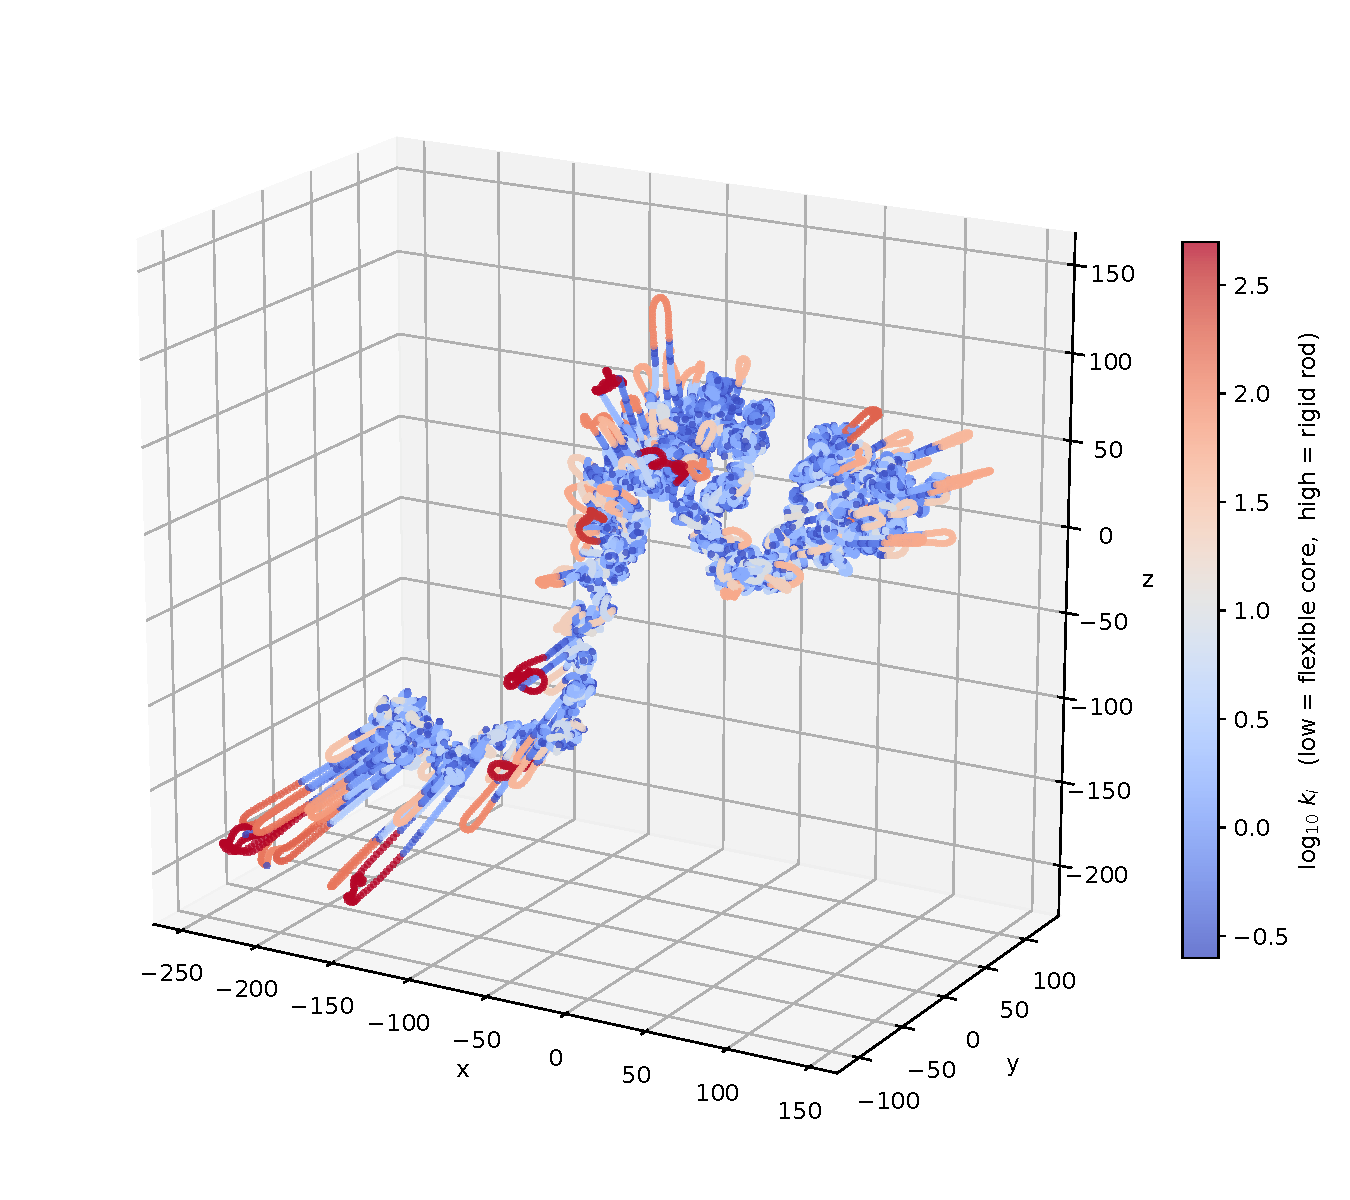
\includegraphics[width=0.72\linewidth]{fig1_conformation.pdf}
\caption{Representative folded conformation of the PDTP chain at $N = 4\times10^{4}$
(overdamped Langevin with simulated annealing, $3800$ steps, seed $42$). Beads are
colored by $\log_{10}$ of the local bending stiffness $k_i$ [Eq.~(1)], from flexible
prime-rich hinges (blue, $k_i = k_{\text{hinge}} = 0.25$) to rigid long-gap rods
(red, capped at $k_{\max} = 500$). The chain collapses to a compact globule
($R_g = 110.7$) in which dense flexible cores are threaded by rigid rods extending
into peripheral loops; for this conformation the stiffness--radius rank correlation
is $\rho = +0.065$ and the tail-weighted core--shell separation $\Delta R = +21.0$.}
\label{fig:conformation}
\end{figure}

\section{Pre-flight calibration}
\label{sec:calib}

Because the stiffness field of Eq.~(1) is amplified exponentially, the rare
long-gap sites carry bending moduli orders of magnitude above the baseline, and an
explicit integrator can in principle diverge within a single step. We bound the
parameters \emph{a priori} through a worst-case stress test on an isolated
segment~\cite{Allen}. We locate the global maximum gap ($g_{\max} = 72$, between the
primes $31397$ and $31469$) and extract the $150$-bead window centred on it
(indices $[31358, 31508)$). The segment is evolved under bond and gap-driven bending
forces alone, with the production displacement cap \emph{removed} so that any latent
divergence is exposed, while a small thermal noise ($k_B T = 0.05$) continually
injects curvature.

Two findings emerge. First, the cosine bending potential of Eq.~(3) is
\emph{self-limiting}: its restoring force scales as $\sin\theta_i$ and vanishes as a
segment straightens, so a rigid rod relaxes toward the straight configuration
without overshoot. Sweeping $\alpha \in [0.05, 0.15]$---and, independently, relaxing
the cap to the fully uncapped limit, where the stiffness at $g_{\max}$ reaches
$k \approx 1.2 \times 10^{4}$ (nearly $5 \times 10^{4}\,k_{\text{hinge}}$)---produces
no divergence over the test window. The exponential amplification is thus \emph{not}
the binding stability constraint. Second, the binding constraint is set by the
stiffest \emph{harmonic} term, the bonds: sweeping the timestep, the scheme is stable
for $\Delta t \le 0.01$ but diverges within a few steps for $\Delta t \gtrsim 0.02$,
consistent with the fastest bond-mode limit $\Delta t \lesssim 2/(4\mu k_{\text{bond}})
\approx 0.011$. Guided by this, the production runs adopt $\alpha = 0.15$ with a
conservative cap $k_{\max} = 500$ (a factor $\approx 25$ below the uncapped worst case)
and a hard displacement bound $\delta_{\max} = 0.25$; with $\Delta t = 0.008$ lying a
factor $\approx 2.5$ below the divergence threshold, all trajectories operate well
inside the stable regime. The calibration's purpose is not to maximize the stiffness
contrast but to certify that the symmetry-breaking map can be integrated without
numerical artifacts that could masquerade as structural signal.

\section{Results}

We compare the true prime chain against surrogates under identical force fields,
dynamics, and annealing; the only difference between arms is the anchor pattern
generating the stiffness field. Three observables characterize the collapsed state:
the radius of gyration $R_g$; the percentile core--shell separation $\Delta R$, the
mean radial distance of the stiffest $20\%$ of beads minus that of the most flexible
$20\%$; and the Spearman rank correlation $\rho$ between local stiffness $k_i$ and
radial distance. Positive $\rho$ or $\Delta R$ indicates rigid segments at the
periphery. Ensembles comprise $n$ independent trajectories per arm.

\subsection{Global collapse is surrogate-invariant}
All arms collapse along indistinguishable trajectories and their gross dimensions do
not separate. At $N = 10^4$ the radius of gyration is $R_g = 57 \pm 16$ (true) versus
$49 \pm 13$ (shuffle) (Welch $p = 0.20$, $n = 10$), and the gross core--shell
amplitude is likewise indistinguishable: $\Delta R = 14.4 \pm 0.7$ versus
$15.1 \pm 0.5$ at $N = 4\times10^4$ ($p = 0.37$, $n = 40$). The overall size and the
gross magnitude of stiffness segregation are therefore fixed by the marginal
stiffness distribution, which every surrogate preserves.

\subsection{A core--shell ordering signature}
The rank correlation $\rho$ reveals a signature of ordering. In our decisive
experiment---$N = 4\times10^4$, deep annealing ($8000$ steps), $n = 40$ per
arm---both arms exhibit positive $\rho$, but the sorting is significantly
\emph{weaker} for the true chain: $\rho = +0.105 \pm 0.007$ versus
$+0.137 \pm 0.004$ (Welch $p = 6.5\times10^{-5}$, Mann--Whitney $p = 3.1\times10^{-4}$,
$d = -0.96$; Fig.~\ref{fig:decisive}). The deterministic ordering thus imposes a
reproducible \emph{resistance} to the radial sorting generic stiff--flexible physics
would otherwise produce. The effect is quantitatively modest---stiffness accounts for
only $\rho^2 \approx 1\%$ of the radial-rank variance---but statistically robust. The
same comparison in $\Delta R$ is not resolved at this size ($p = 0.37$): the ordering
signal resides in the global rank structure, not in the stiffness extremes, which is
why the low-variance estimator $\rho$ is required.

\begin{figure}[htbp]
\centering
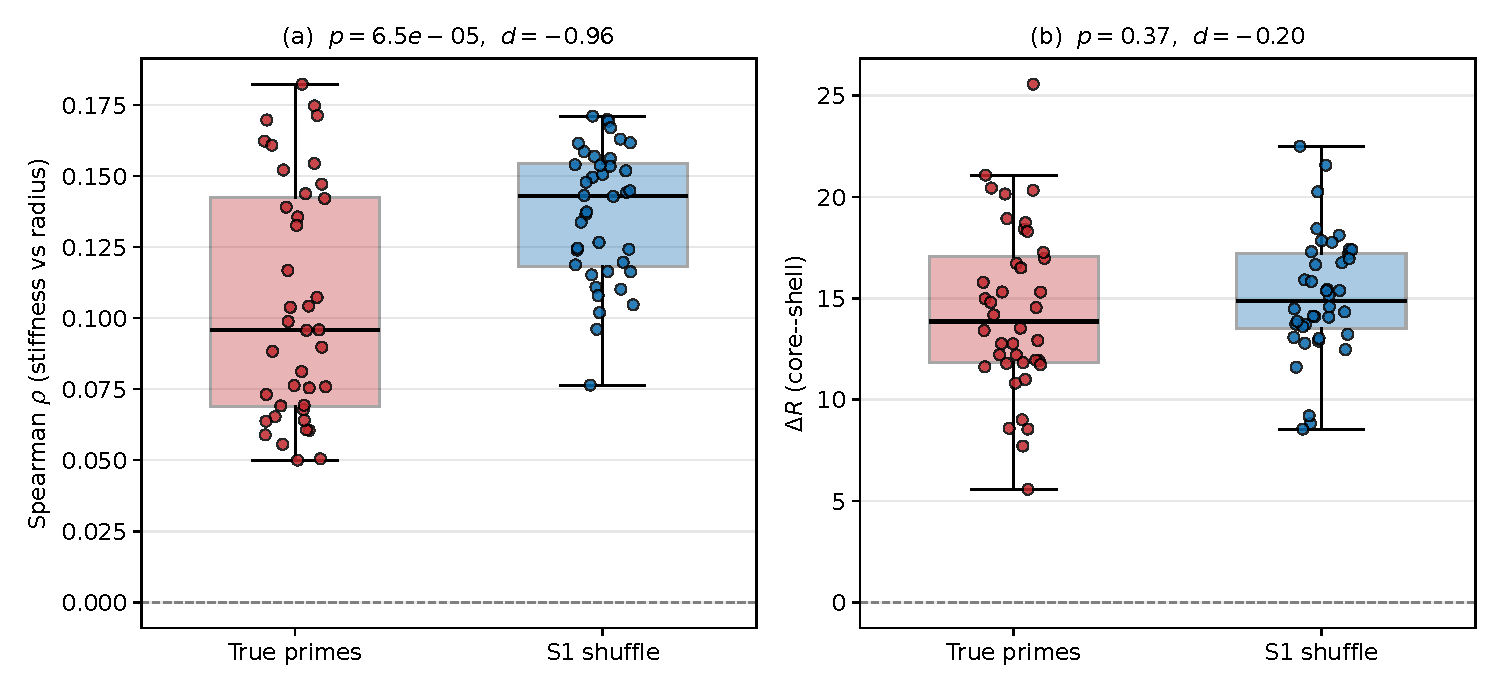
\includegraphics[width=0.92\linewidth]{fig2_decisive.pdf}
\caption{Decisive test at $N = 4\times10^{4}$, deep annealing ($8000$ steps),
$n = 40$ per arm. (a)~Spearman $\rho$: true primes $+0.105 \pm 0.007$ vs.\ shuffle
S1 $+0.137 \pm 0.004$ (Welch $p = 6.5\times10^{-5}$, Mann--Whitney
$p = 3.1\times10^{-4}$, $d = -0.96$)---the true sequence is significantly less
radially sorted. (b)~$\Delta R = 14.4 \pm 0.7$ vs.\ $15.1 \pm 0.5$ ($p = 0.37$,
$d = -0.20$), statistically indistinguishable. Boxes: median and quartiles; points:
individual runs.}
\label{fig:decisive}
\end{figure}

\subsection{Ordering versus marginal distribution}
To attribute the effect we compare three arms at $N = 10^4$, $n = 40$: the true
chain; the Shuffle (S1), preserving the exact gap multiset but randomizing order; and
a Cram\'er surrogate (S3), placing pseudo-primes at density $1/\ln i$, preserving only
the coarse density trend~\cite{Cramer}. The decomposition is clean
(Fig.~\ref{fig:decomp}). The ordering contrast (true vs.\ S1) is strongly significant
($\Delta\rho = -0.051$, $p = 1.6\times10^{-5}$, $d = -1.05$). The marginal-shape
contrast (S1 vs.\ S3), both order-randomized, is small and not significant
($\Delta\rho = -0.017$, $p = 0.09$, $d = -0.38$). The combined contrast (true vs.\ S3)
is largest ($\Delta\rho = -0.068$, $p = 1.2\times10^{-6}$, $d = -1.18$). Arithmetic
ordering therefore accounts for the bulk of the effect ($\approx 75\%$ of the combined
shift), while the shape of the gap distribution contributes little. This is the
central result: what the folded conformation registers is not the composition of the
prime-gap sequence but its sequential, long-range arithmetic structure.

\begin{figure}[htbp]
\centering
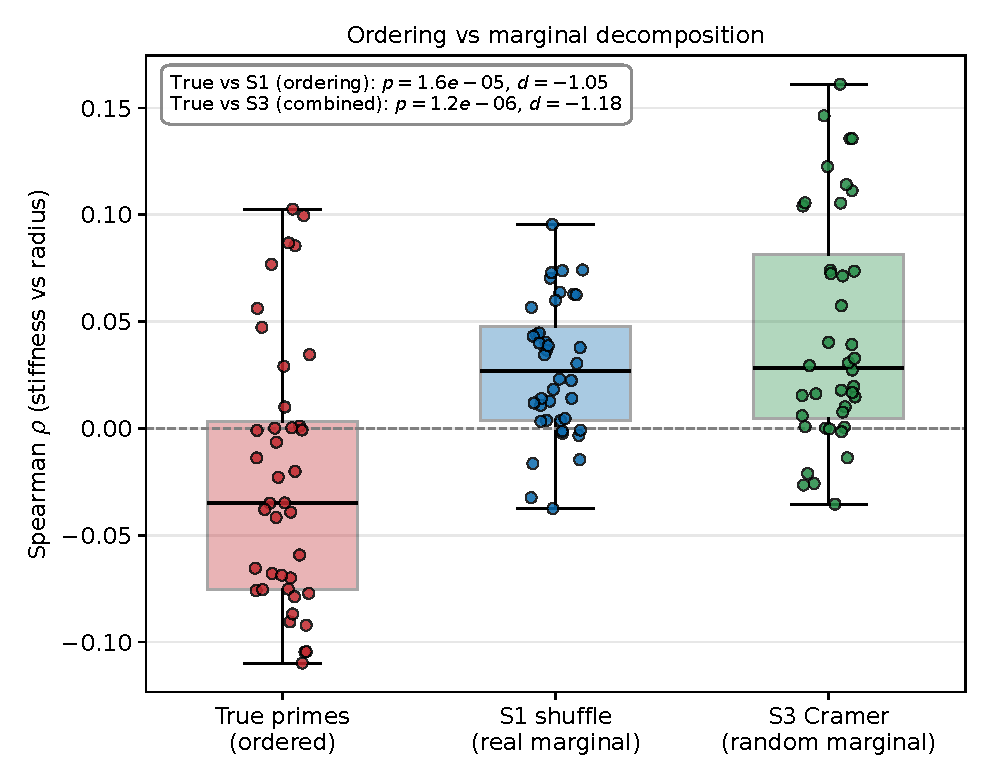
\includegraphics[width=0.6\linewidth]{fig3_decomposition.pdf}
\caption{Ordering versus marginal-distribution decomposition at $N = 10^{4}$,
$n = 40$ per arm. True primes ($\rho = -0.023 \pm 0.010$), shuffle S1
($+0.028 \pm 0.005$; exact gap multiset, order randomized), and Cram\'er surrogate S3
($+0.045 \pm 0.009$; pseudo-primes at density $1/\ln i$). Ordering (true vs.\ S1):
$p = 1.6\times10^{-5}$, $d = -1.05$. Marginal shape (S1 vs.\ S3): $p = 0.09$
(n.s.). Combined (true vs.\ S3): $p = 1.2\times10^{-6}$, $d = -1.18$.}
\label{fig:decomp}
\end{figure}

\subsection{Finite-size behaviour}
Finally, we examine the size dependence across $N = 10^4, 2\times10^4, 4\times10^4$
(Fig.~\ref{fig:fss}). In both $\rho$ and $\Delta R$, the true chain lies
systematically below the shuffle at every size, with significance at $N = 10^4$ and
$2\times10^4$ ($\rho$: $p = 3\times10^{-3}$ and $2\times10^{-3}$). An initial sweep at
$N = 4\times10^4$ with reduced statistics ($n = 20$) and shallower annealing returned
a gap below threshold ($p = 0.075$); the decisive experiment of Sec.~4.2 shows this to
be a power-and-protocol artifact rather than a genuine fade---at matched per-bead
annealing depth and $n = 40$, the same gap is recovered at $p = 6.5\times10^{-5}$. We
caution that the \emph{absolute} correlation grows with $N$ for both arms (from
$\rho \approx 0$ at $N = 10^4$ to $\rho \approx +0.1$ at $N = 4\times10^4$), reflecting
both progressive collapse and the varying annealing depth of the sweep; consequently
only the fixed-$N$ gap between true and shuffle constitutes a controlled comparison,
and we read the absolute $N$-dependence as a trend rather than an equilibrium scaling
law. Within the range studied, once statistics and annealing depth are controlled, the
ordering signature is present and significant at every size.

\begin{figure}[htbp]
\centering
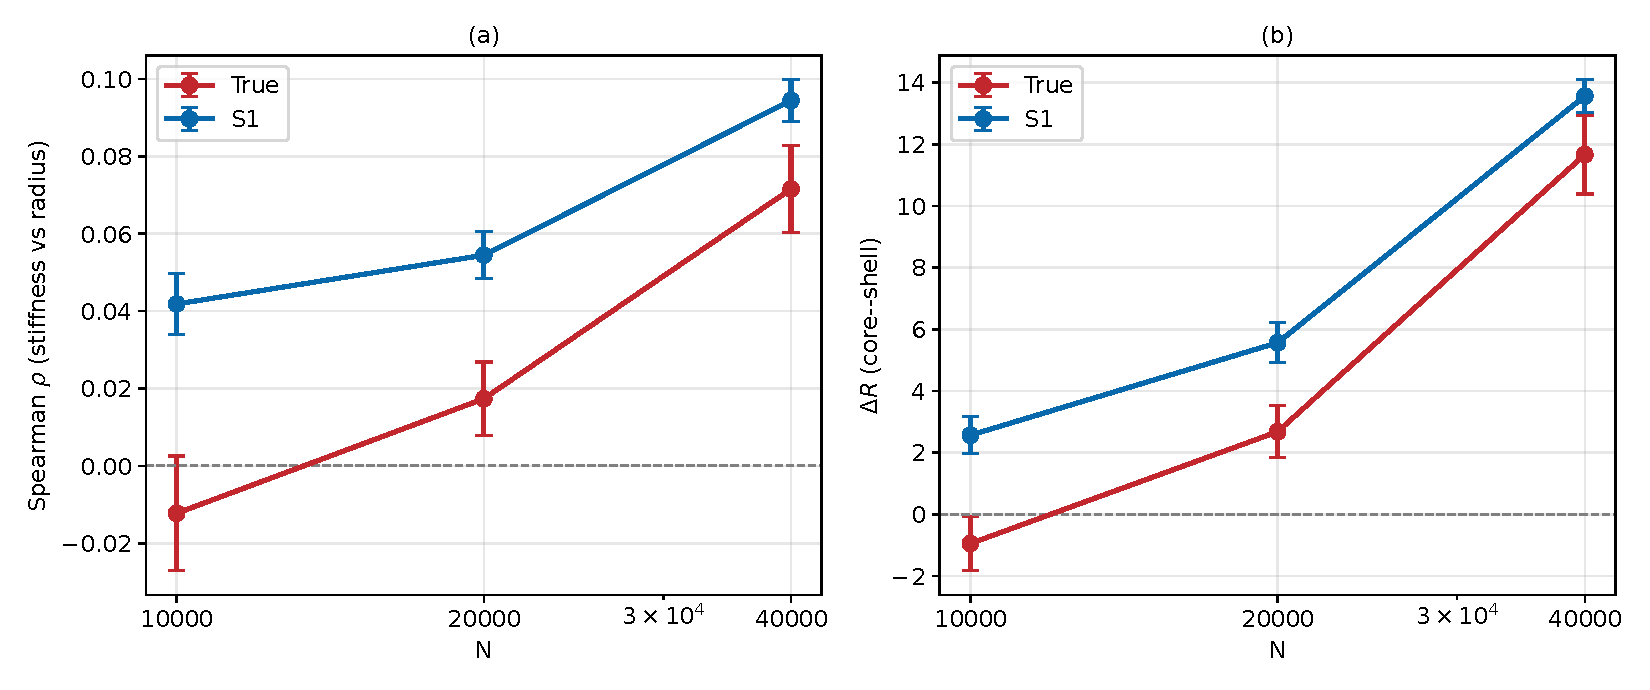
\includegraphics[width=0.92\linewidth]{fig4_finite_size.pdf}
\caption{Finite-size behaviour, true vs.\ shuffle S1, for
$N = 10^{4}, 2\times10^{4}, 4\times10^{4}$ ($n = 20$ per arm; annealing
$2000/3500/5000$ steps). (a)~Spearman $\rho$ and (b)~$\Delta R$ vs.\ $N$
(mean $\pm$ s.e.m.). The true chain lies below the shuffle at every size. The gap is
significant at $N = 10^{4}$ and $2\times10^{4}$; the reduced-statistics point at
$N = 4\times10^{4}$ ($p = 0.075$) is resolved by the deeper-annealed, higher-$n$
experiment of Fig.~\ref{fig:decisive} ($p = 6.5\times10^{-5}$). Only the fixed-$N$
true--shuffle gap is a controlled comparison.}
\label{fig:fss}
\end{figure}

\section{Discussion}

\subsection{What the fold registers}
The representative conformation (Fig.~\ref{fig:conformation}; $R_g \approx 111$)
displays the generic architecture of a semiflexible heteropolymer: dense flexible
cores threaded and flanked by rigid rods that extend into loops toward the periphery.
Both the true chain and its surrogates share this gross morphology; their difference
lies elsewhere. Neither $R_g$ nor $\Delta R$ distinguishes the true sequence from a
stiffness-matched shuffle; only the rank correlation $\rho$ does, and there the true
sequence is significantly \emph{less} sorted. The folded conformation thus behaves as
a physical readout sensitive not to the composition of the stiffness sequence but to
its sequential arrangement---specifically to correlations that a random permutation
destroys.

\subsection{A candidate mechanism}
Why should ordering matter once the chain has collapsed? We advance a concrete,
falsifiable hypothesis. In the true sequence the long gaps are not placed
independently: prime gaps carry documented correlations and
clustering~\cite{HardyLittlewood,AresCastro}, superposed on a weak positional drift.
We conjecture that this correlated placement embeds a fraction of the rigid rods
within flexible neighborhoods, impeding their migration to the surface and thereby
\emph{reducing} the stiffness--radius correlation relative to a sequence in which the
identical rods are scattered independently. Concretely, the abundance of small gaps
---twin primes (gap $2$) alone account for ${\approx}14\%$ of all gaps at
$N = 4\times10^4$---creates local clusters of flexible hinges~\cite{HardyLittlewood},
which we hypothesize act as \emph{topological traps} that anchor neighboring rigid
rods within the interior and oppose their radial expulsion. The hypothesis is directly testable with
scale-selective surrogates---for instance a block-preserving permutation that retains
local gap order within contiguous segments while scrambling their large-scale
arrangement, and its converse---which would localize the correlation length
responsible for the signal. The present data establish that ordering matters, not yet
how.

\subsection{Connections}
Our result offers a physical manifestation of the fact that the prime-gap sequence is
neither periodic nor memoryless~\cite{HardyWright,HardyLittlewood,AresCastro}: a
folding process, despite the drastic coarse-graining it imposes, still transmits a
residue of arithmetic order into three-dimensional structure. In this sense the
polymer acts as an unconventional probe of long-range correlations in the primes,
complementary to spectral and combinatorial approaches~\cite{Montgomery,BerryKeating}.
On the physical side, the construction sits within the study of aperiodic and
deterministic order---quasicrystals, aperiodic tilings, and sequence-programmed
matter~\cite{Shechtman,Levine,Macia}. We are, however, cautious about extrapolation:
the effect is small in absolute terms, and we make no claim of a route to functional
metamaterials. What we demonstrate is narrower and cleaner: that a deterministic,
aperiodic arithmetic sequence leaves a detectable, reproducible imprint on the
equilibrium-like conformation of a physical model, distinguishable from every
marginal-matched null.

\subsection{Limitations}
Several limitations bound these conclusions. First, the effect is quantitatively
small: local stiffness accounts for only $\sim\!1\%$ of the radial-rank variance, the
distributions overlap heavily, and no single conformation can be classified as
``prime'' or ``shuffled''---the signal is a shift in the ensemble mean. Second, our
ensembles are generated by simulated annealing rather than sampled from a true
equilibrium distribution; absolute observables depend on the protocol, and only the
fixed-$N$ true--surrogate contrast, annealed identically, is controlled. Third, we
have examined a single stiffness map---one $\alpha$, one functional form, one
confinement; robustness across this parameter space remains to be charted. Fourth, our
sizes reach only $N = 4\times10^4$; the absolute correlation drifts upward with $N$,
and while the gap is significant at every size once statistics and annealing depth are
controlled, its fate in the thermodynamic limit is genuinely open. Finally, the signal
is carried by the sensitive rank estimator $\rho$ and is not resolved by the tail-based
$\Delta R$ at the largest size. We emphasize that this is a controlled in-silico
construction: we make no claim that prime numbers are physically privileged in nature,
and none of biological relevance.

\section{Conclusion}
We introduced the PDTP model and used it to ask whether the folded state of an
aperiodic-but-deterministic sequence is determined by its composition alone or also by
its arithmetic ordering. By comparing the true prime chain against surrogates that
preserve the marginal stiffness distribution exactly while destroying order, we found
the answer to be affirmative but bounded. The gross conformation is
surrogate-invariant---neither $R_g$ nor $\Delta R$ distinguishes true from shuffle---so
overall size and coarse morphology are fixed by the marginal distribution. The finer
organization is not: the stiffness--radius rank correlation is significantly suppressed
for the true sequence ($\rho = +0.105$ vs.\ $+0.137$ at $N = 4\times10^4$;
$p = 6.5\times10^{-5}$, $d = -0.96$), an effect a three-way decomposition attributes to
arithmetic ordering rather than to the gap distribution, and reproducible across sizes
once statistics and annealing depth are controlled. The effect is quantitatively
modest ($\sim\!1\%$ of the radial-rank variance) and is a property of the ensemble
rather than of any single fold. Beyond the specific case of primes, the PDTP framework
and its surrogate-null methodology offer a controlled testbed for how one-dimensional
deterministic order is---and is not---expressed in three-dimensional structure. The
most immediate directions are to resolve the correlation scale responsible for the
signal through scale-selective surrogates, to map the effect across the stiffness-map
parameter space, and to determine its fate at system sizes well beyond those reached
here.

\section*{Data and code availability}
All code, data, and figure-generation scripts that reproduce the results of this paper
are openly available at
\url{https://github.com/Ruqing1963/prime-driven-topological-polymer}. The repository
contains the pre-flight calibration, the surrogate/null-model decomposition, the
finite-size sweep, the decisive $N = 4\times10^4$ experiment, and the conformation
generator, together with the ensemble result files and a script that regenerates all
figures.

\begin{thebibliography}{99}
\bibitem{deGennes} P.-G. de Gennes, \emph{Scaling Concepts in Polymer Physics}
(Cornell University Press, Ithaca, 1979).
\bibitem{LiebermanAiden} E. Lieberman-Aiden \emph{et al.}, Science \textbf{326}, 289 (2009). \href{https://doi.org/10.1126/science.1181369}{doi:10.1126/science.1181369}.
\bibitem{Pande} V. S. Pande, A. Yu. Grosberg, and T. Tanaka, Rev. Mod. Phys. \textbf{72}, 259 (2000). \href{https://doi.org/10.1103/RevModPhys.72.259}{doi:10.1103/RevModPhys.72.259}.
\bibitem{Leibler} L. Leibler, Macromolecules \textbf{13}, 1602 (1980). \href{https://doi.org/10.1021/ma60078a047}{doi:10.1021/ma60078a047}.
\bibitem{Bates} F. S. Bates and G. H. Fredrickson, Annu. Rev. Phys. Chem. \textbf{41}, 525 (1990). \href{https://doi.org/10.1146/annurev.pc.41.100190.002521}{doi:10.1146/annurev.pc.41.100190.002521}.
\bibitem{Bryngelson} J. D. Bryngelson and P. G. Wolynes, Proc. Natl. Acad. Sci. USA \textbf{84}, 7524 (1987). \href{https://doi.org/10.1073/pnas.84.21.7524}{doi:10.1073/pnas.84.21.7524}.
\bibitem{Garel} T. Garel and H. Orland, Europhys. Lett. \textbf{6}, 307 (1988). \href{https://doi.org/10.1209/0295-5075/6/4/005}{doi:10.1209/0295-5075/6/4/005}.
\bibitem{Montgomery} H. L. Montgomery, in \emph{Analytic Number Theory}, Proc. Sympos. Pure Math. \textbf{24}, 181 (1973).
\bibitem{BerryKeating} M. V. Berry and J. P. Keating, SIAM Rev. \textbf{41}, 236 (1999). \href{https://doi.org/10.1137/S003614459834749X}{doi:10.1137/S003614459834749X}.
\bibitem{Shechtman} D. Shechtman, I. Blech, D. Gratias, and J. W. Cahn, Phys. Rev. Lett. \textbf{53}, 1951 (1984). \href{https://doi.org/10.1103/PhysRevLett.53.1951}{doi:10.1103/PhysRevLett.53.1951}.
\bibitem{Levine} D. Levine and P. J. Steinhardt, Phys. Rev. Lett. \textbf{53}, 2477 (1984). \href{https://doi.org/10.1103/PhysRevLett.53.2477}{doi:10.1103/PhysRevLett.53.2477}.
\bibitem{HardyWright} G. H. Hardy and E. M. Wright, \emph{An Introduction to the Theory of Numbers}, 6th ed. (Oxford University Press, Oxford, 2008).
\bibitem{Cramer} H. Cram\'er, Acta Arith. \textbf{2}, 23 (1936). \href{https://doi.org/10.4064/aa-2-1-23-46}{doi:10.4064/aa-2-1-23-46}.
\bibitem{Macia} E. Maci\'a, Rep. Prog. Phys. \textbf{69}, 397 (2006). \href{https://doi.org/10.1088/0034-4885/69/2/R03}{doi:10.1088/0034-4885/69/2/R03}.
\bibitem{KratkyPorod} O. Kratky and G. Porod, Recl. Trav. Chim. Pays-Bas \textbf{68}, 1106 (1949). \href{https://doi.org/10.1002/recl.19490681203}{doi:10.1002/recl.19490681203}.
\bibitem{Montesi} A. Montesi, M. Pasquali, and F. C. MacKintosh, Phys. Rev. E \textbf{69}, 021916 (2004). \href{https://doi.org/10.1103/PhysRevE.69.021916}{doi:10.1103/PhysRevE.69.021916}.
\bibitem{WCA} J. D. Weeks, D. Chandler, and H. C. Andersen, J. Chem. Phys. \textbf{54}, 5237 (1971). \href{https://doi.org/10.1063/1.1674820}{doi:10.1063/1.1674820}.
\bibitem{Ermak} D. L. Ermak and J. A. McCammon, J. Chem. Phys. \textbf{69}, 1352 (1978). \href{https://doi.org/10.1063/1.436761}{doi:10.1063/1.436761}.
\bibitem{Kirkpatrick} S. Kirkpatrick, C. D. Gelatt, and M. P. Vecchi, Science \textbf{220}, 671 (1983). \href{https://doi.org/10.1126/science.220.4598.671}{doi:10.1126/science.220.4598.671}.
\bibitem{Allen} M. P. Allen and D. J. Tildesley, \emph{Computer Simulation of Liquids}, 2nd ed. (Oxford University Press, Oxford, 2017).
\bibitem{HardyLittlewood} G. H. Hardy and J. E. Littlewood, Acta Math. \textbf{44}, 1 (1923). \href{https://doi.org/10.1007/BF02403921}{doi:10.1007/BF02403921}.
\bibitem{AresCastro} S. Ares and M. Castro, Physica A \textbf{360}, 285 (2006). \href{https://doi.org/10.1016/j.physa.2005.05.045}{doi:10.1016/j.physa.2005.05.045}.
\end{thebibliography}

\end{document}
